\documentclass{beamer}

\newcommand{\lang}{\stackrel{\rightarrow}{\mathcal{L}}}

%\usepackage{pgf,pgfarrows,pgfnodes,pgfautomata,pgfheaps,pgfshade,newalg}
%\usepackage{epic}
%\usepackage{eepic}
%\usepackage{epsf}
%\usepackage{boxedminipage}

\usepackage[T1]{fontenc}
\usepackage[cp1250]{inputenc}

%\usepackage[usenames,dvipsnames]{xcolor}

\setbeamertemplate{background canvas}[vertical shading][]

%\setbeamertemplate{itemize item}[ball]

%\usetheme{warsaw}
%\usebackgroundtemplate{\includegraphics[width=\paperwidth, height=\paperheight]{FrontexTemplate.jpg}}
\usefonttheme[onlysmall]{structurebold}
\usecolortheme[named=blue]{structure}


\definecolor{darkblue}{RGB}{0,51,153}

\definecolor{darkgreen}{RGB}{0,110,0}
  

\setbeamertemplate{frametitle}
{
\vspace{0.3cm}\hspace{-0.5cm}
\color{darkblue}
\textbf{\insertframetitle}
\par
}

\setbeamertemplate{navigation symbols}{}

\definecolor{gold}{rgb}{0.85,.66,0}

\bibliographystyle{alpha}


\title{{Balto-Slavic Natural Language Processing 2017}}

\date{{\color{white} 4 April 2017, Valencia, Spain}}

\begin{document}

%\maketitle

%\usebackgroundtemplate{\includegraphics[width=\paperwidth, height=\paperheight]{AutomatedEventExtraction_firstPage.jpg}}
%\begin{frame}[plain]
%
%\end{frame}

\begin{frame}[fragile]
 \frametitle{}

\center{{\color{blue} \Large{\textbf{6-th Workshop\\on\\Balto-Slavic Natural Language Processing}}}}

\vspace{0.3cm}

\center{{\color{blue} \large{4 April 2017\\ Valencia, Spain}}}

\vspace{0.3cm}

\center{{\color{black} \normalsize{SPONSORED BY}}}

\vspace{-0.2cm}

\begin{figure}[h!]
    \centering\leavevmode
    %\hspace{1cm}
    
\includegraphics[scale=0.55]{sigslav.png}
\end{figure} 

\end{frame}

\begin{frame}[fragile]
 \frametitle{Some statistics ...}

\begin{itemize}

\item \textbf{26 submissions: 24 regular + 2 shared task system descriptions}

\item accepted 14 regular papers and 2 shared task system descriptions \verb+->+  \textbf{acceptance rate: 58\%}

\item 3 reviews per paper

\item PC response: ~99\%

\item \textbf{topics:} 2 papers relate to \textbf{lexical semantics}, 4 to \textbf{development of
linguistic resources}, 4 to \textbf{IF, IR, and IE}, 4 cover topics related to processing of \textbf{non-standard language} 
or \textbf{user-generated content}, and one paper describes the Challenge.

\item \textbf{language coverage:} Croatian (7), Czech (1), Lithuanian (1), Polish (3), Russian (5), Russyn (1), Serbian (2), Slovak (1), Slovene (4) and Ukrainian (1).

\end{itemize}

\end{frame}

\begin{frame}[fragile]
 \frametitle{More statistics ... (Origin of the authors)}

\begin{figure}[h!]
    \centering\leavevmode
    \hspace{1cm}
    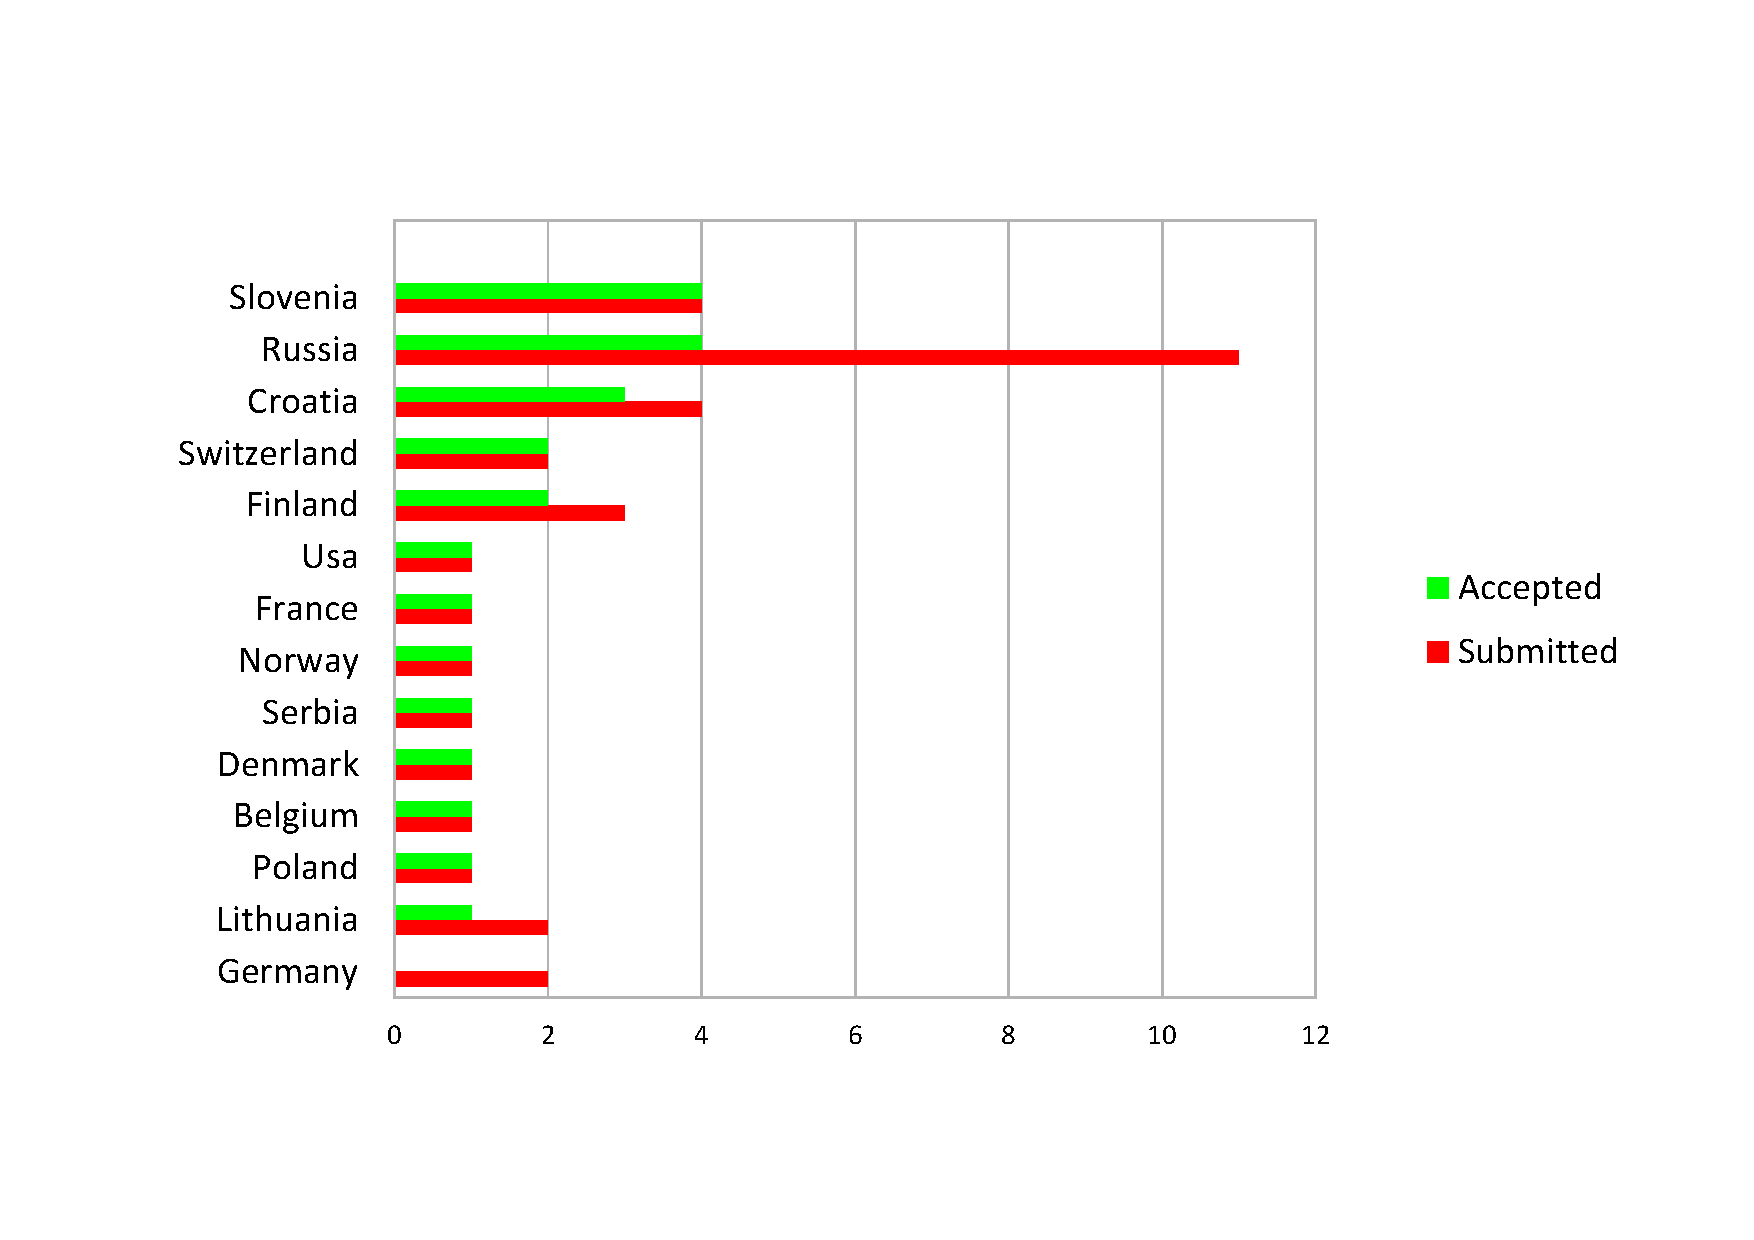
\includegraphics[scale=0.38]{stats.pdf}
\end{figure} %

\end{frame}


%\usebackgroundtemplate{\includegraphics[width=\paperwidth, height=\paperheight]{wordle.png}}


%\begin{frame}
% \frametitle{}

%\end{frame}

%\usebackgroundtemplate{\includegraphics[width=\paperwidth, height=\paperheight]{white.png}}


\begin{frame}
 \frametitle{Programme}

\begin{itemize}

\item[9:10] INVITED TALK: \textit{Serge Sharoff}

\item[10:00] Session I: Lexical Semantics

\item[11:00] {\color{darkgreen}Coffee Break}

\item[11:30] Session II: Development of Linguistic Resources

\item[13:10] {\color{darkgreen}Lunch Break}

\item[14:30] Session III: Processing Non-Standard Language and User-Generated Content

\item[16:10] {\color{darkgreen}Coffee Break}

\item[16:30] Session IV: Shared Task on Multilingual Named Entity Recognition

\item[17:20] Session V: Information Filtering, Retrieval, and Extraction

\item[18:40] END 

\end{itemize}

\end{frame}

\begin{frame}[fragile]
\frametitle{SIGSLAV Elections}

\begin{itemize}
\item All elected officers of the SIG shall be elected by a vote of the membership
\item SIGSLAV Officers:
\begin{itemize}
\item Chair
\item Vice-Chair
\item Secretary
\item Resource Managers
\end{itemize}
\item The term of all elected officers is two years or shorter, if the elected officers organize the elections earlier
\end{itemize}
\end{frame}

\begin{frame}[fragile]
 \frametitle{SIGSLAV Elections}

\begin{itemize}

	\item[17 Apr] 1st call for nominations

	\item[8 May] 2nd call for nominations

	\item[22 May] Nominations close

	\item[5 Jun] Sending out queries to candidates to confirm nominations

	\item[7 Aug] Voting commences

	\item[11 Sep] Voting ends

	\item[18 Sep] Announcement of the elected officers

	\item[1 Nov] Elected officers start their service
\end{itemize}

\end{frame}



\begin{frame}[fragile]
 \frametitle{Feedback \& Contact}

\textbf{email:} {\color{blue} \large{\verb+bsnlp@cs.helsinki.fi+}}

\vspace{1cm}

\textbf{web}: {\color{blue} \large{\verb+http://bsnlp-2017.cs.helsinki.fi+}}

\vspace{1cm}

\textbf{SIGSLAV}: {\color{blue} \large{\verb+http://sigslav.cs.helsinki.fi+}}


\end{frame}


\end{document}
